\documentclass[12pt, xcolor={svgnames,table}]{beamer}
%\documentclass[20pt,handout]{beamer}
\usetheme{Darmstadt}
\usepackage{graphicx}
%\usepackage[german]{babel}
\usepackage{ngerman}
\usepackage[T1]{fontenc}
\usepackage[utf8]{inputenc}
\usepackage{tikz}
\setbeamertemplate{footline}[frame number]

\newcommand{\cc}[1]{\includegraphics[height=4mm]{img/#1.png}\hspace{1mm}}
\usepackage{ifthen}
\newcommand{\license}[2][]{\\#2\ifthenelse{\equal{#1}{}}{}{\\\scriptsize\url{#1}}}
\usepackage{textcomp}
\usepackage{hyperref}
%\usepackage[table]{xcolor}

\pgfdeclareimage[height=.6cm]{c3d2logo}{./img/c3d2.pdf}

\pgfdeclarelayer{foreground}
\pgfsetlayers{main,foreground}
\logo{\pgfputat{\pgfxy(-1,0)}{\pgfbox[center,base]{\pgfuseimage{c3d2logo}}}}

\title{Smartphonesicherheit}
\author{\small Marius Melzer (marius@rasumi.net) \\\large Chaos Computer Club Dresden}
\date{15.03.2016}

\begin{document}
\maketitle

\section{Einleitung}
\subsection{}

\begin{frame}
    \frametitle{Chaos Computer Club}
    \begin{center}
	
\includegraphics[height=0.2\textheight]{img/chaosknoten.png}
    \end{center}	
    \begin{itemize}
      \item<1-> Verein wurde 1981 gegr"undet (\url{https://ccc.de})
      \item<2-> Aktuell > 6000 Mitglieder
      \item<3-> Technologie zum gesellschaftlichen Nutzen (und nicht ihrem Schaden)
      \item<4-> Betreibt u.a. "Offentlichkeitsarbeit und Politikberatung
    \end{itemize}
\end{frame}

\begin{frame}
  \frametitle{Chaos Computer Club}
  \begin{figure}
    
\includegraphics[height=0.7\textheight]{img/fingerabdruck.jpg}
  \end{figure}
\end{frame}

\begin{frame}
  \frametitle{Chaos Computer Club}
  \begin{figure}
    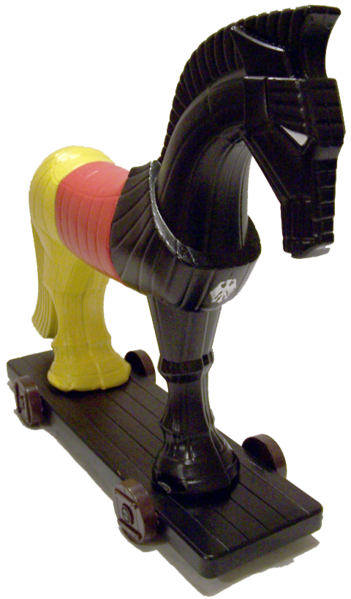
\includegraphics[height=0.7\textheight]{img/trojaner.png}
  \end{figure}
\end{frame}

\begin{frame}
    \frametitle{Chaos Computer Club}
    \begin{center}
	
\includegraphics[height=0.1\textheight]{img/c3d2_logo.png}
    \end{center}
    \begin{itemize}
      \item<1-> Chaos Computer Club Dresden (\url{https://c3d2.de})
      \item<2-> Datenspuren: Herbst 2016 (\url{https://datenspuren.de})
      \item<3-> Podcasts (\url{https://c3d2.de/radio.html})
      \item<4-> Chaos macht Schule (\url{https://c3d2.de/schule.html})
    \end{itemize}
\end{frame}

\begin{frame}
    \frametitle{Bundespräsident Gauck zur NSA-Überwachung}
    \begin{center}
      ``Wir wissen z.B., dass es nicht so ist, wie bei der Stasi und dem KGB, dass es dicke Aktenbände gibt, wo unsere Gesprächsinhalte alle aufgeschrieben und schön abgeheftet sind. Das ist es nicht.''
      (Gauck, 30.06.2013 im ZDF-Sommerinterview)
    \end{center}
\end{frame}

\begin{frame}
    \frametitle{Stasi vs. NSA}
    \begin{center}
      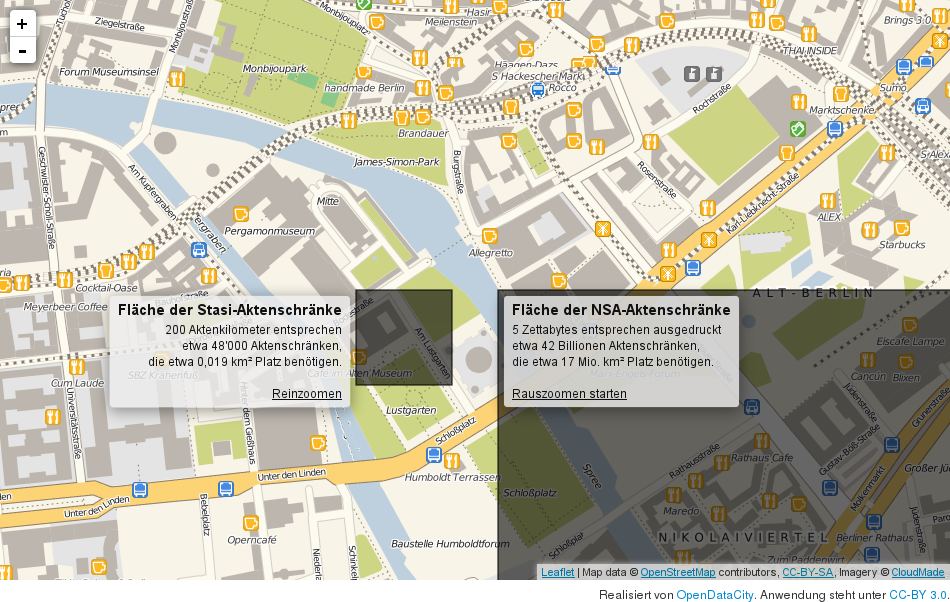
\includegraphics[height=0.7\textheight]{img/akten1.png}
    \end{center}
\end{frame}

\begin{frame}
    \frametitle{Stasi vs. NSA}
    \begin{center}
      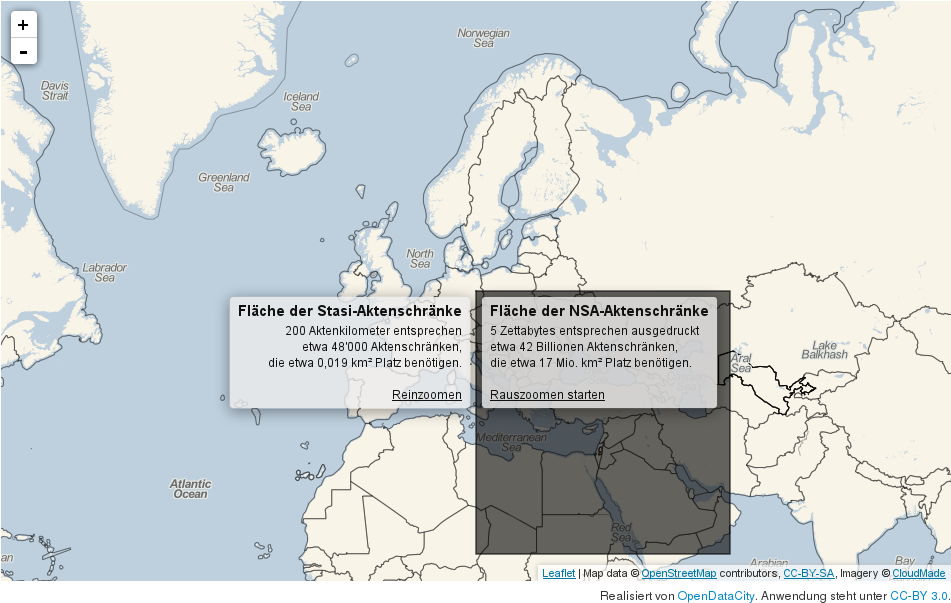
\includegraphics[height=0.7\textheight]{img/akten2.png}
    \end{center}
\end{frame}

\begin{frame}
    \frametitle{``Ich hab ja nichts zu vergergen''}
    \begin{center}
      ``Arguing that you don't care about the right to privacy because you have nothing to hide is no different than saying you don't care about free speech because you have nothing to say. ''
      (Edward Snowden, 21.05.2015 auf Reddit)
    \end{center}
\end{frame}

\begin{frame}
    \frametitle{Samsung vs. 1984}
    \begin{center}
      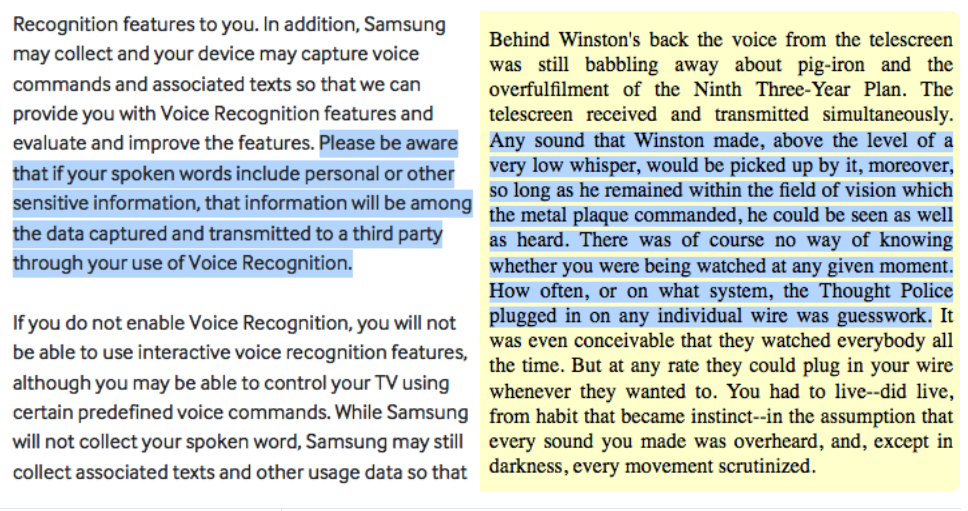
\includegraphics[height=0.7\textheight]{img/samsung-1984.png}
    \end{center}
\end{frame}

\section{Einführung}
\subsection{}

\begin{frame}
    \frametitle{Wie kommunizieren wir im Internet?}
    \begin{center}
      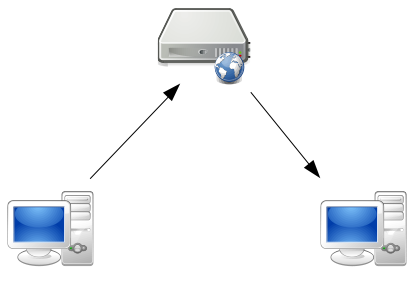
\includegraphics[height=5cm]{img/c-s.png}
    \end{center}
\end{frame}

\begin{frame}
    \frametitle{Server im Rechenzentrum}
    \begin{center}
      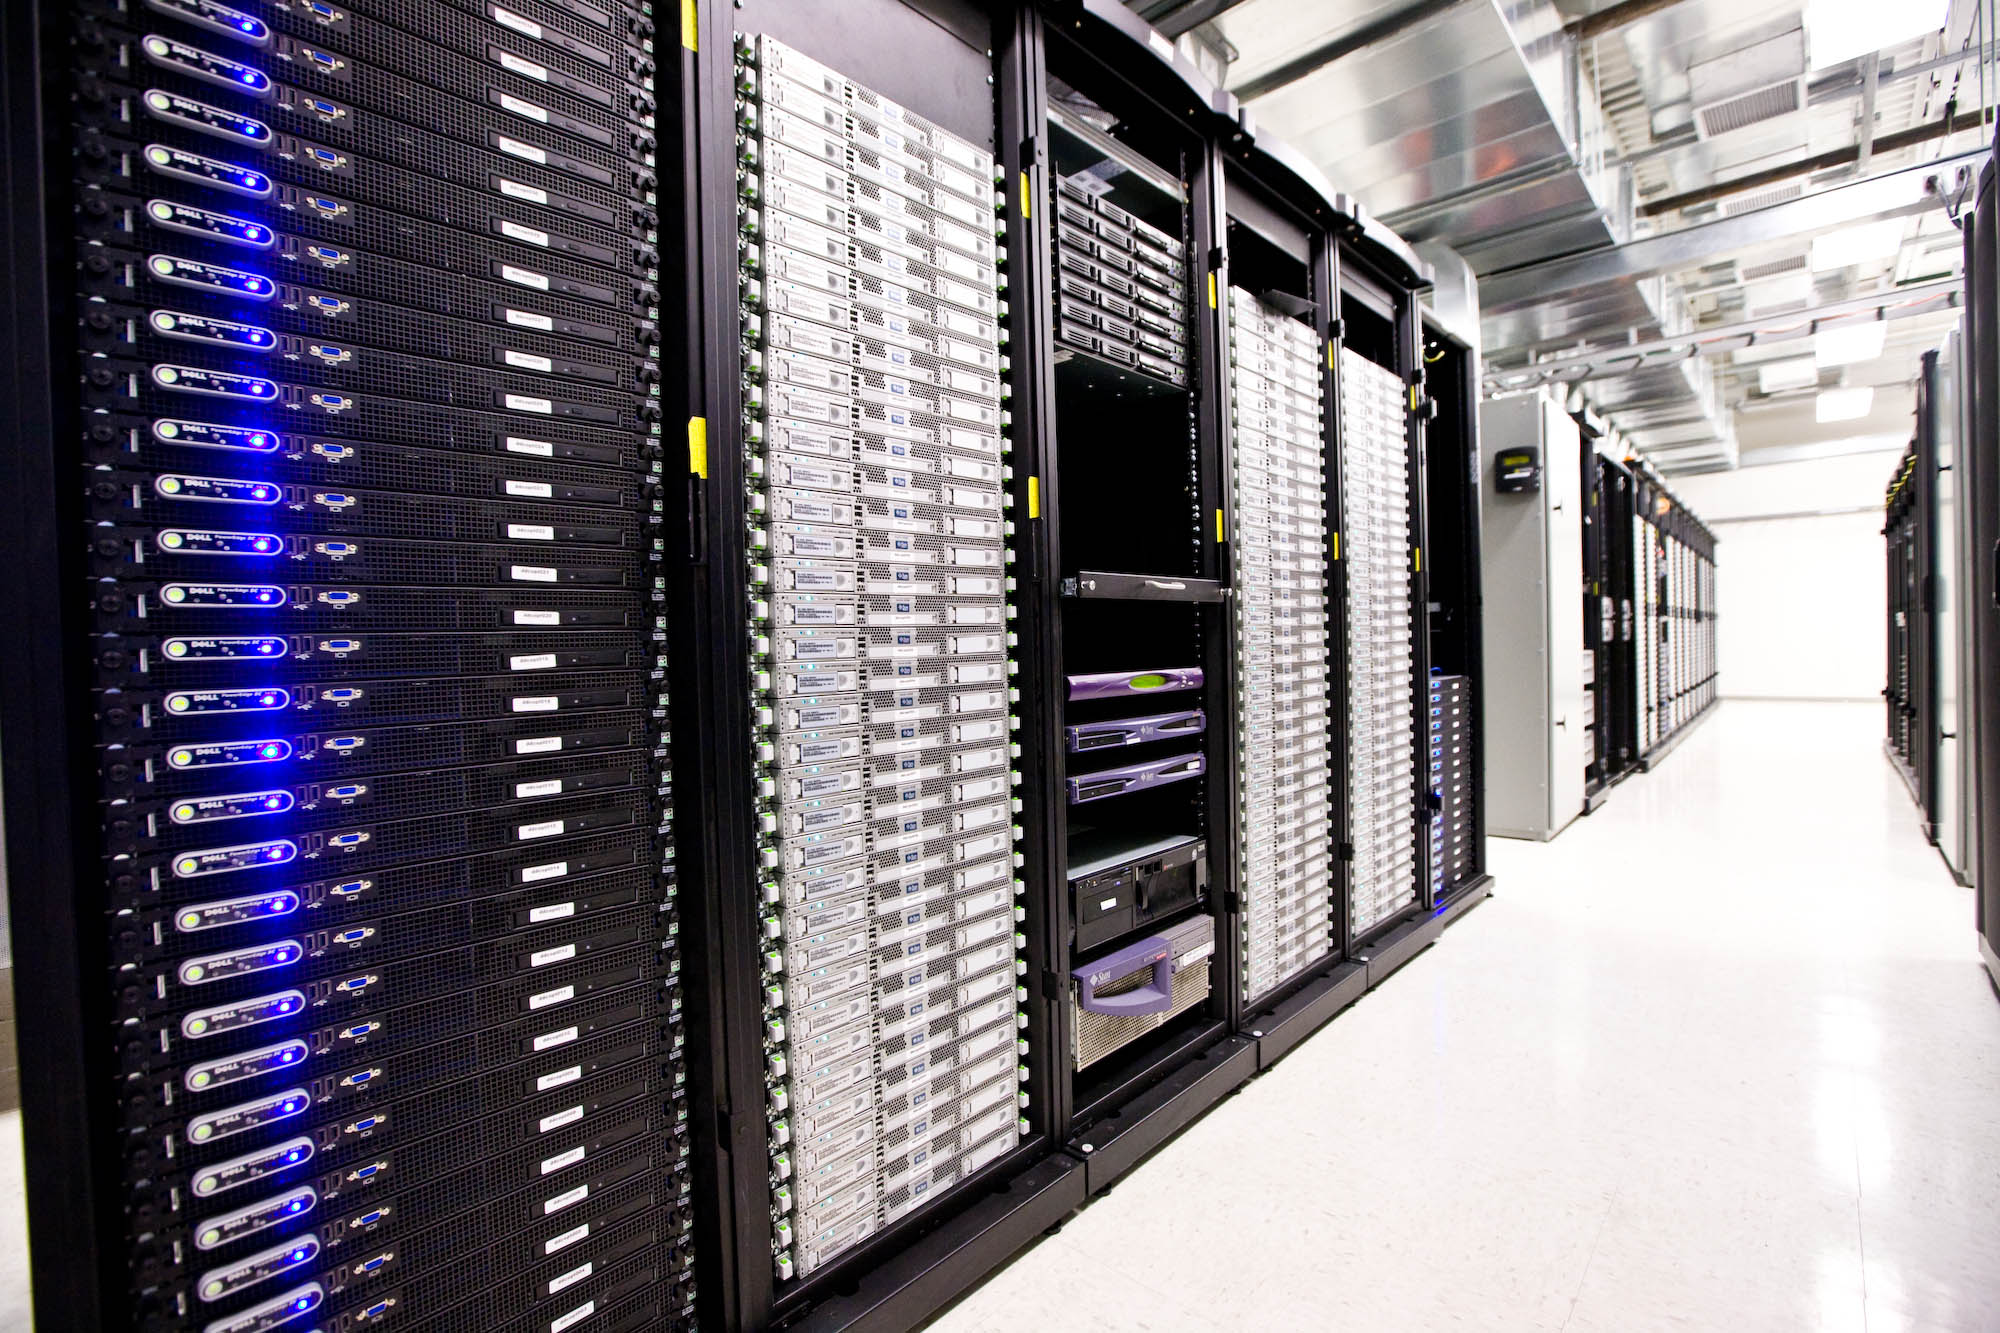
\includegraphics[height=5cm]{img/data_center.jpg}
    \end{center}
\end{frame}

\begin{frame}
    \frametitle{Internetknoten (Router)}
    \begin{center}
      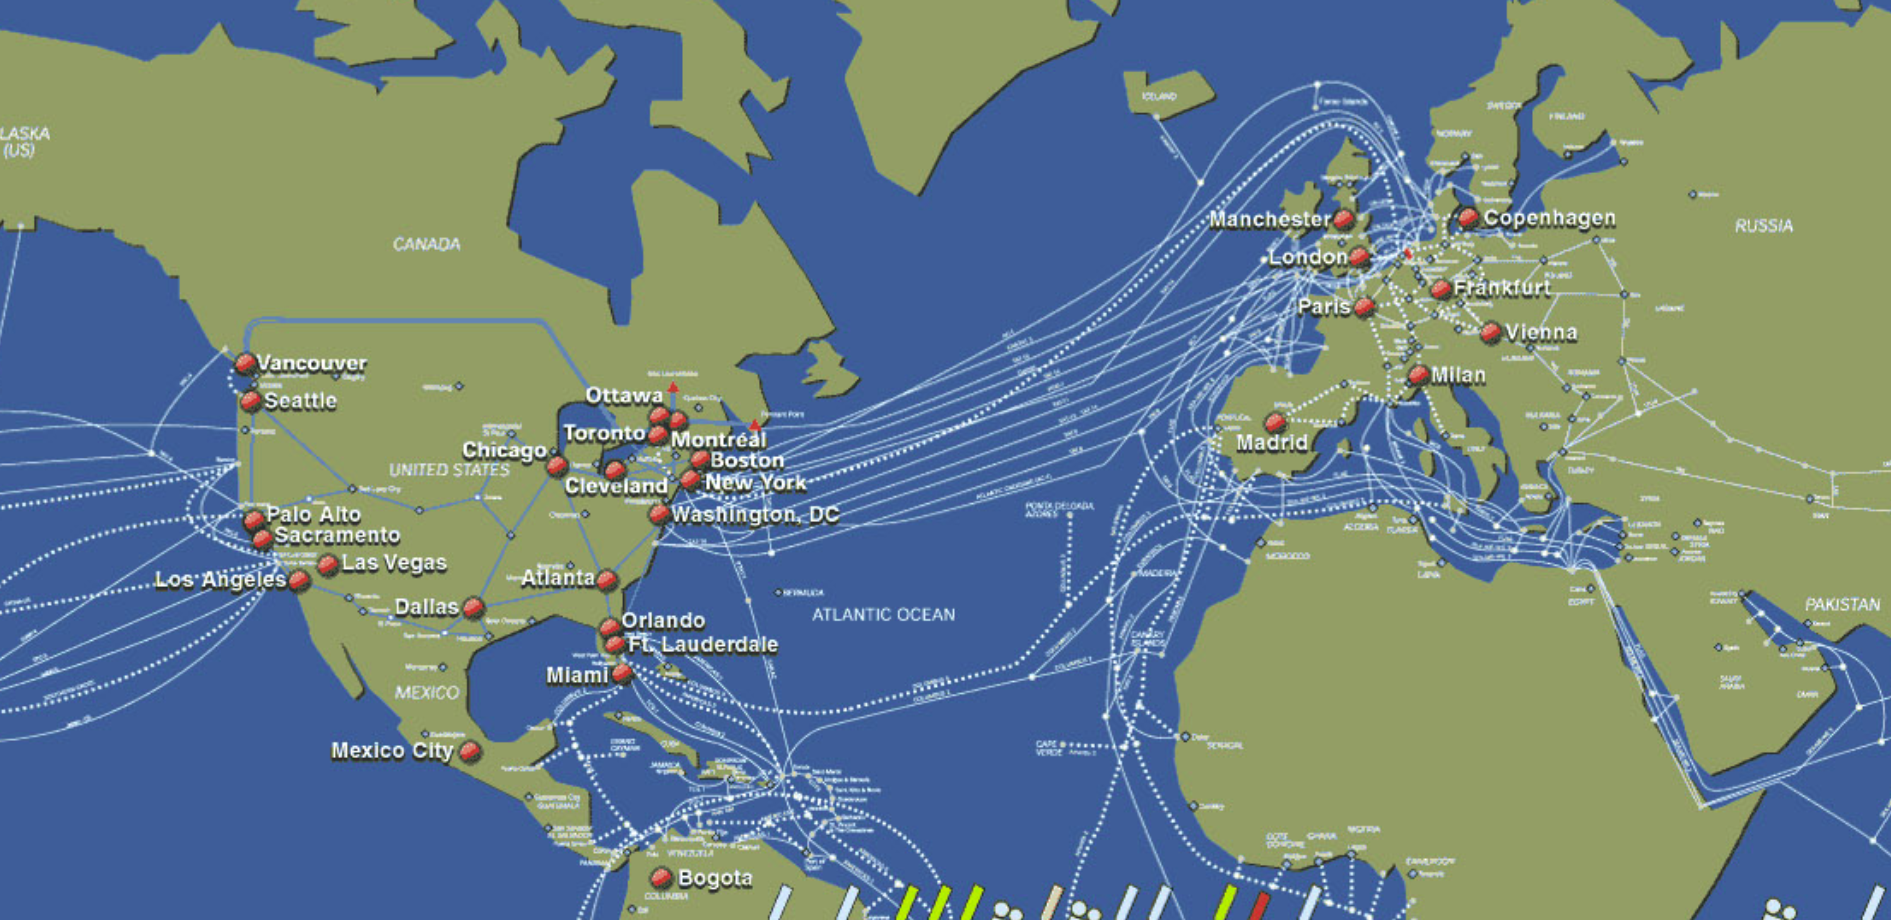
\includegraphics[height=5cm]{img/internet_cable_map.png}
    \end{center}
\end{frame}

\begin{frame}
    \frametitle{Internetknoten (DE-CIX in Frankfurt)}
    \begin{center}
      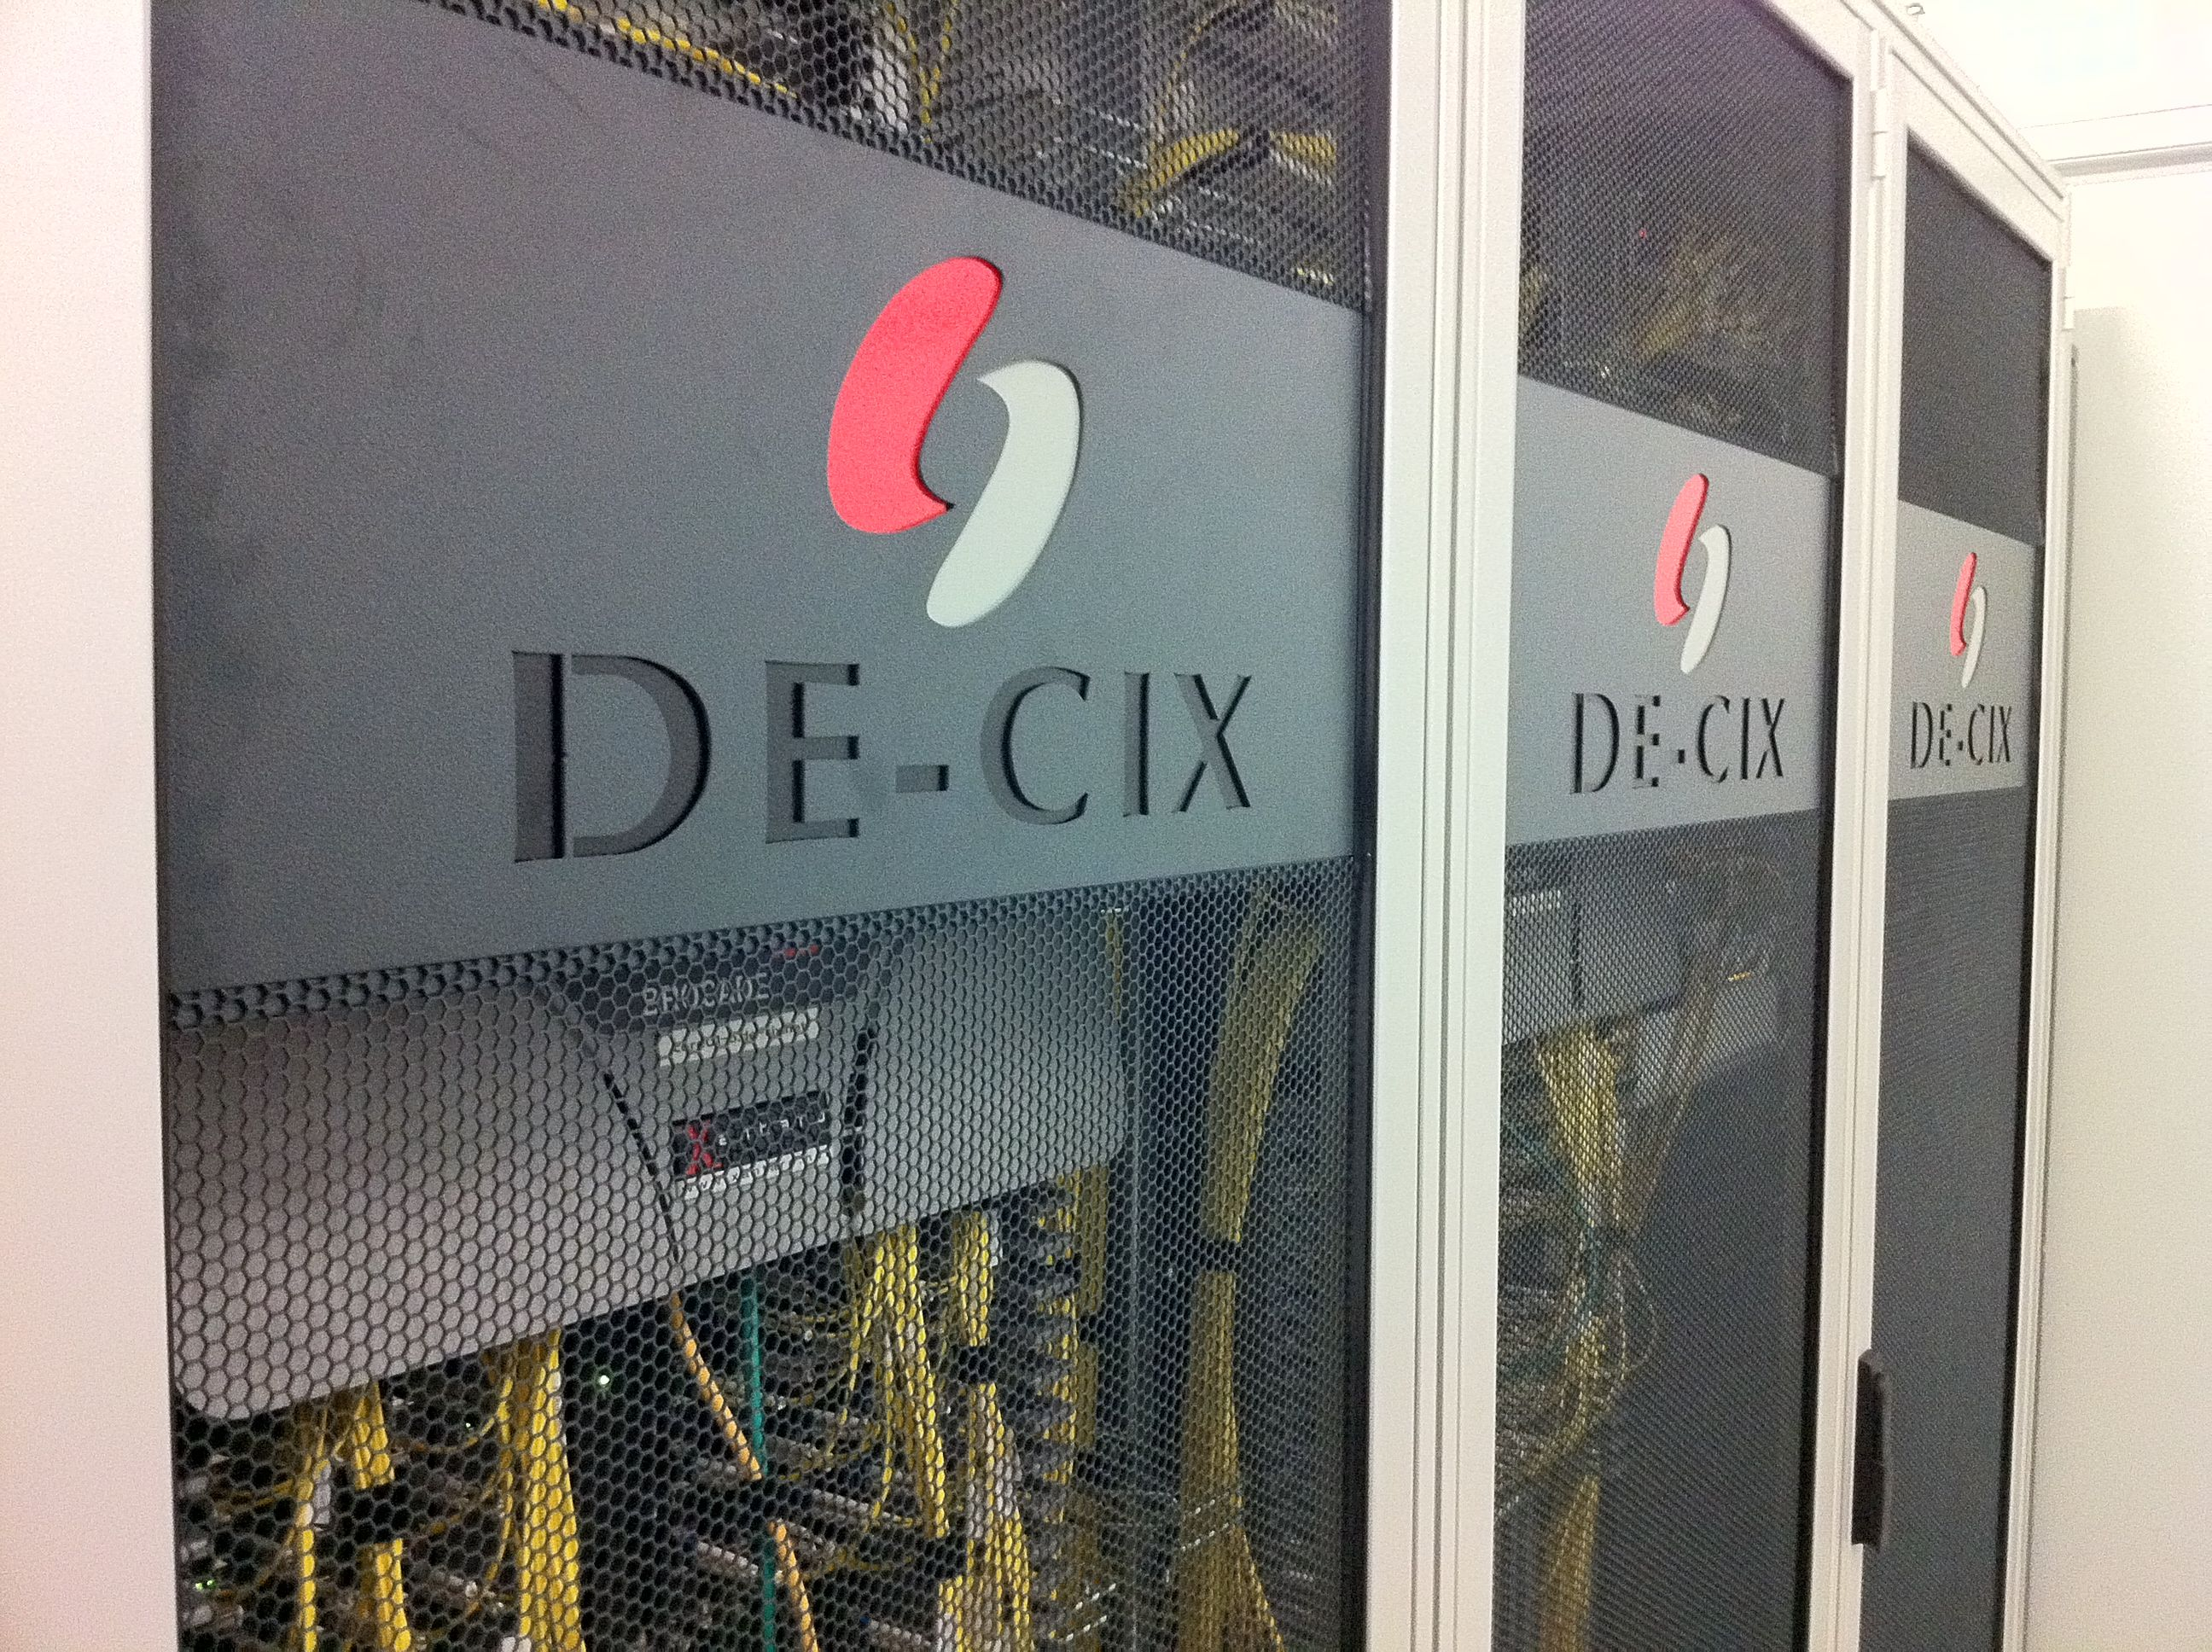
\includegraphics[height=5cm]{img/de_cix.jpg}
      \\{\small \href{https://de.wikipedia.org/wiki/DE-CIX\#/media/File:DE-CIX\_GERMANY\_-\_Switch\_Rack\_\%286218137120\%29.jpg}{Grafik}: \href{https://creativecommons.org/licenses/by-sa/2.0/}{\cc{by-sa} Stefan Funke}}
    \end{center}
\end{frame}

\begin{frame}
    \frametitle{Was ist zu schützen?}
    \begin{center}
      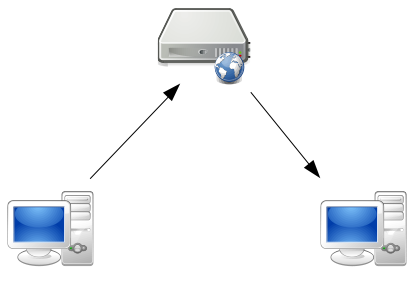
\includegraphics[height=5cm]{img/c-s.png}
    \end{center}
\end{frame}

\section{Geräte}
\subsection{}

\begin{frame}
  \frametitle{Problematisches Verhalten von Software}
  \begin{itemize}
    \item<2-> Sicherheitslücken
    \item<3-> Backdoors
    \item<4-> Unerwünschte Funktionalität
  \end{itemize}
\end{frame}

\begin{frame}
  \frametitle{Schwachstellen}
  \begin{center}
    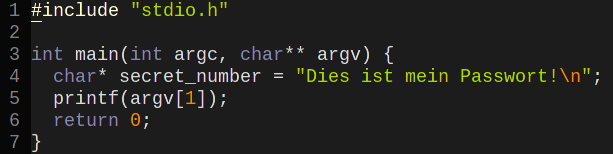
\includegraphics[width=10cm]{img/formatstring.png}
  \par\end{center}
\end{frame}

\begin{frame}
  \frametitle{Größe von Softwareprojekten}
  \begin{center}
    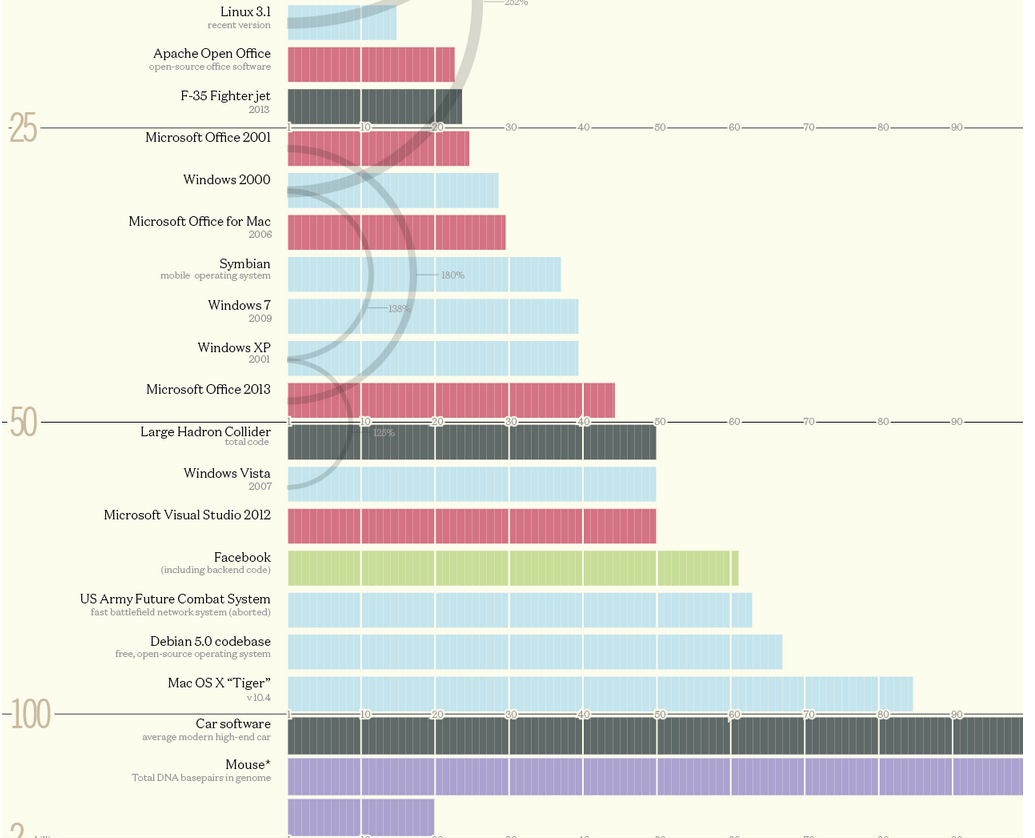
\includegraphics[width=10cm]{img/linesofcode.png}
  \par\end{center}
\end{frame}

\begin{frame}
  \frametitle{Größe von Softwareprojekten}
  \begin{center}
    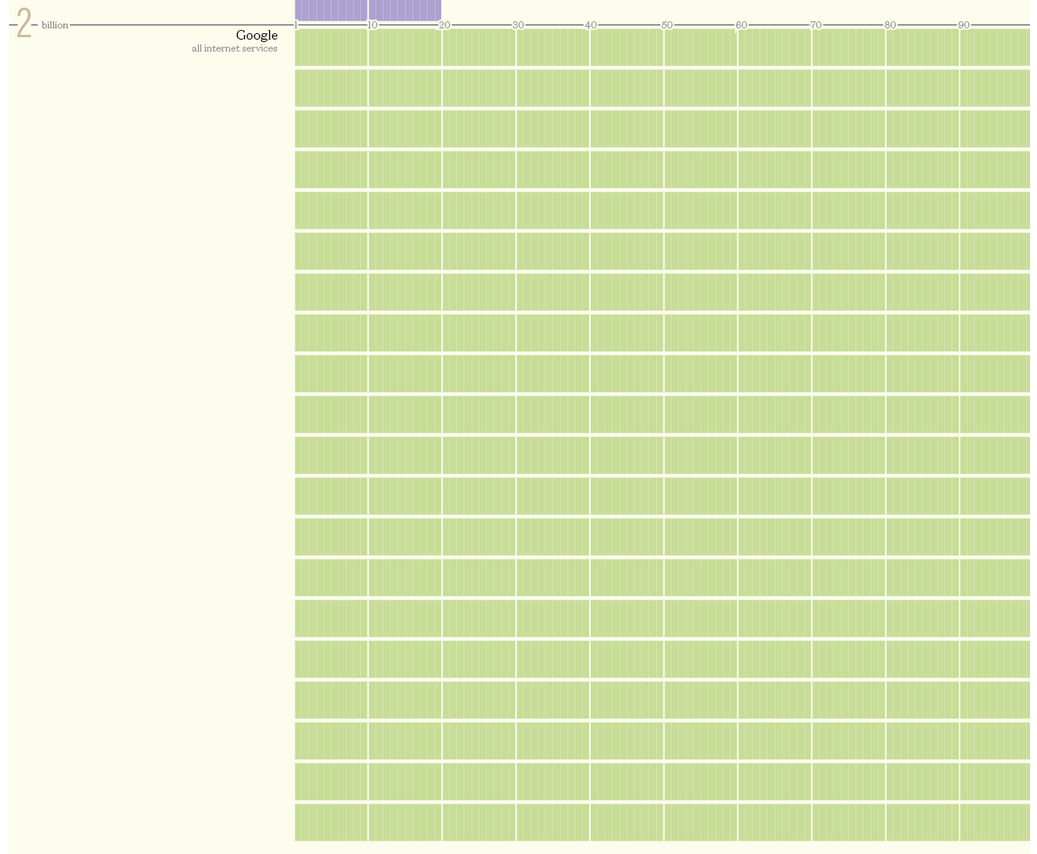
\includegraphics[width=10cm]{img/linesofcode-google.png}
  \par\end{center}
\end{frame}

\begin{frame}
  \frametitle{Backdoors}
  \begin{center}
    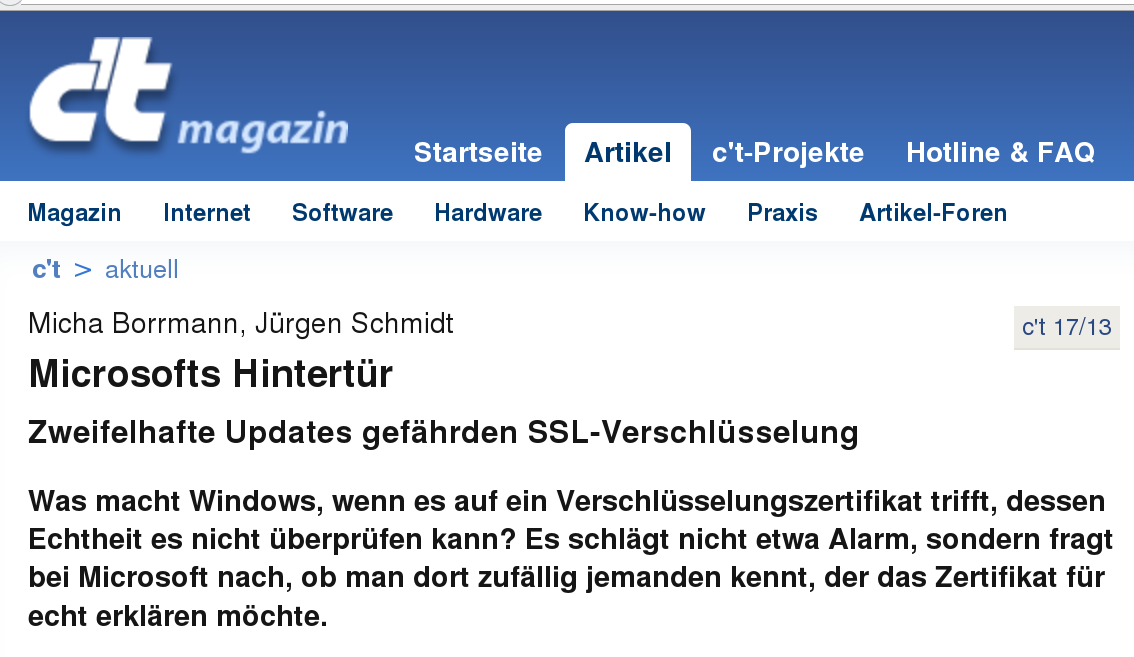
\includegraphics[width=10cm]{img/backdoor-windows}
  \par\end{center}
\end{frame}

\begin{frame}
  \frametitle{Backdoors}
  \begin{center}
    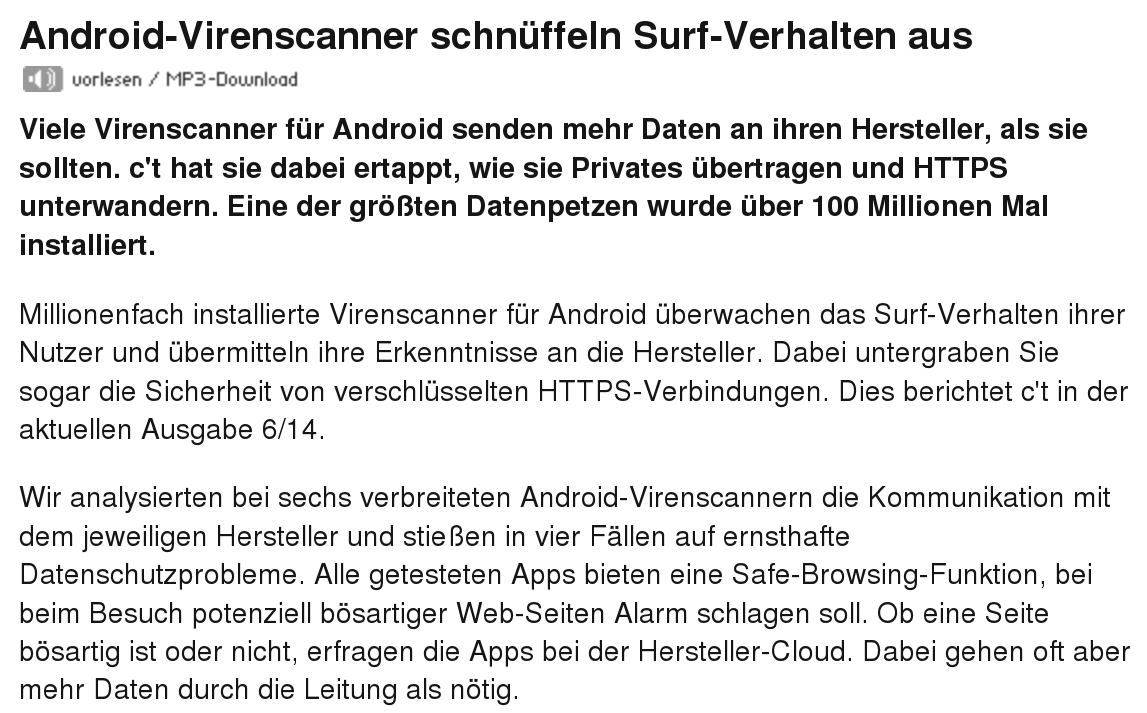
\includegraphics[width=10cm]{img/backdoor-av}
  \par\end{center}
\end{frame}

\begin{frame}
  \frametitle{Backdoors (politische Debatte)}
  \begin{center}
    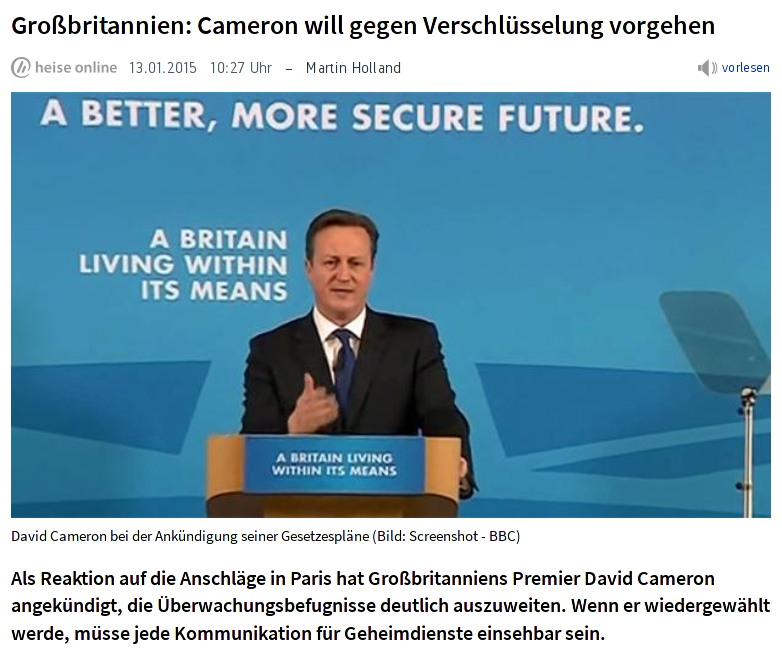
\includegraphics[width=10cm]{img/backdoor_gb.png}
  \par\end{center}
\end{frame}

\begin{frame}
    \frametitle{Unerwünschte Funktionalität}
    \begin{center}
      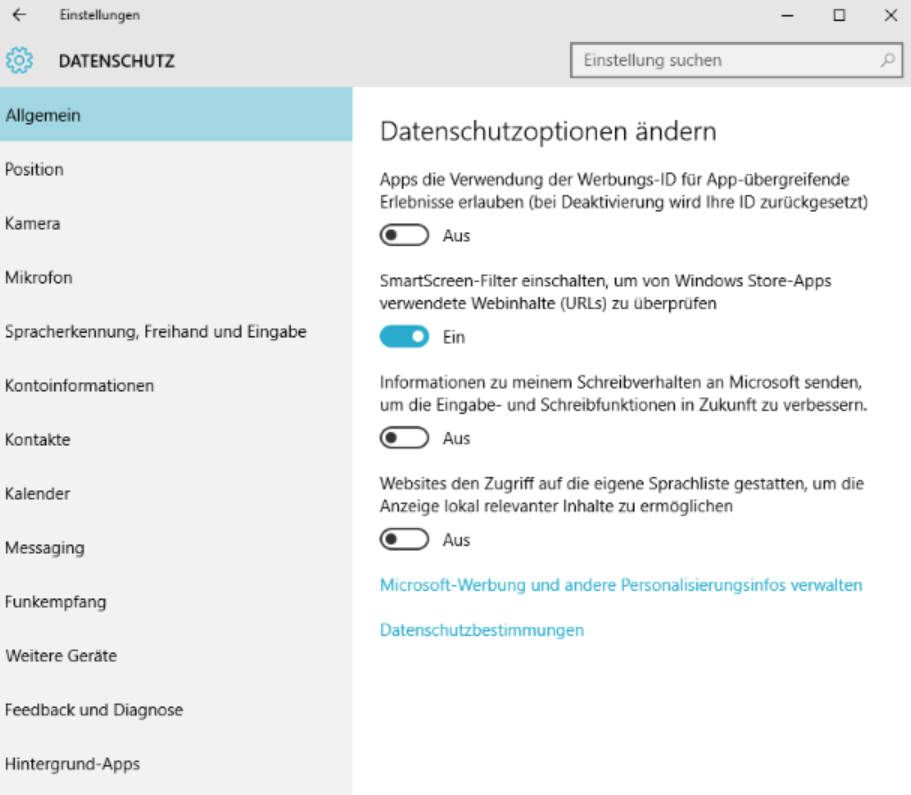
\includegraphics[width=0.7\textwidth]{img/windows10.png}
    \end{center}
\end{frame}

\begin{frame}
  \frametitle{Unerwünschte Funktionalität}
  \begin{center}
    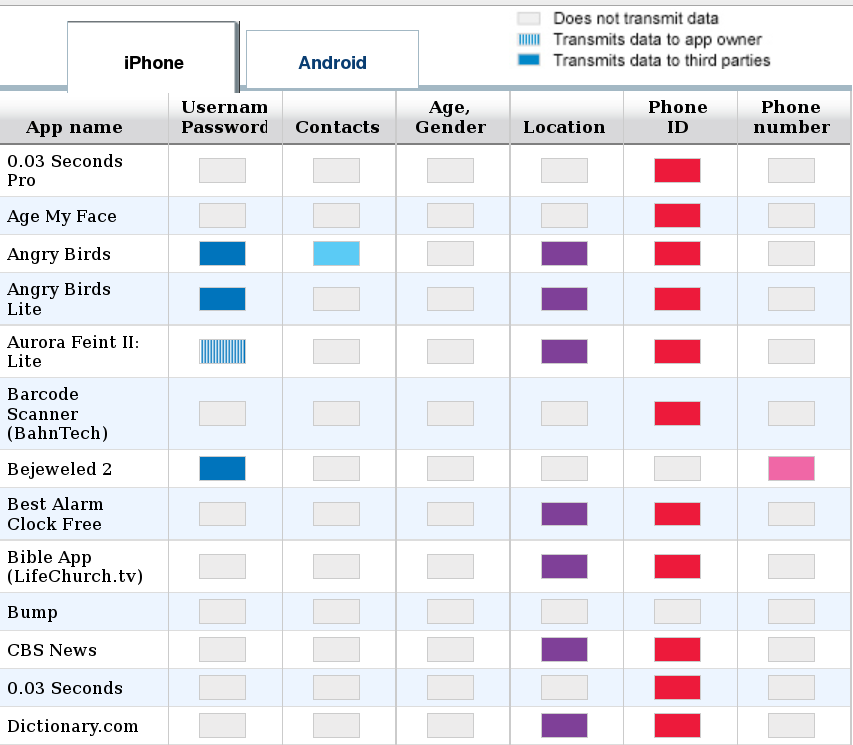
\includegraphics[width=7cm]{img/backdoor-apps}
  \par\end{center}
\end{frame}

\begin{frame}
  \frametitle{Unerwünschte Funktionalität}
  \begin{center}
    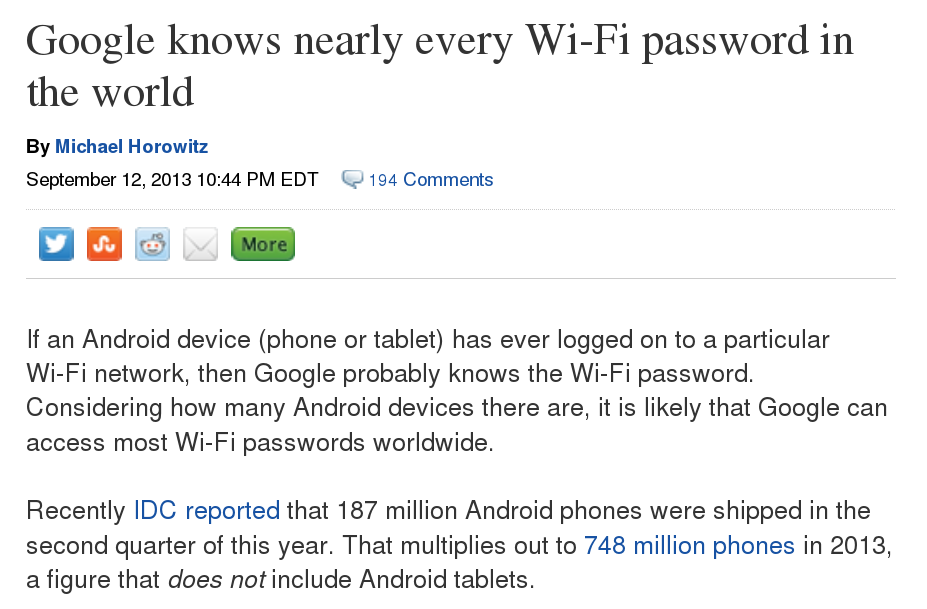
\includegraphics[width=10cm]{img/backdoor-android}
  \par\end{center}
\end{frame}

\begin{frame}
  \frametitle{Unerwünschte Funktionalität}
  \begin{center}
    ``Tie all of our products together, so we further lock customers into our ecosystem'' (Steve Jobs)
  \end{center}
\end{frame}

\begin{frame}
  \frametitle{Unerwünschte Funktionalität}
  \begin{center}
    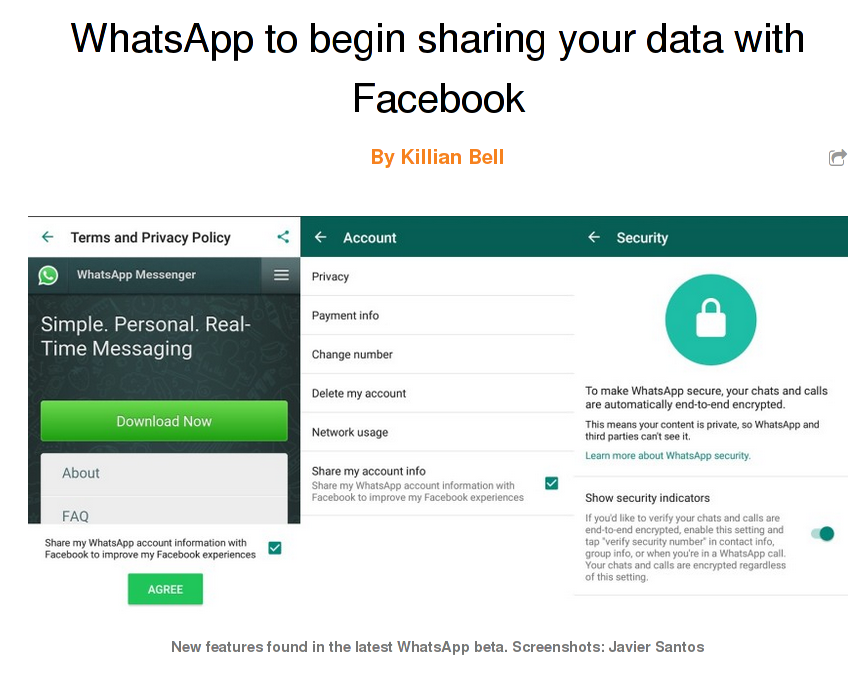
\includegraphics[width=10cm]{img/facebook_whatsapp.png}
  \par\end{center}
\end{frame}

\begin{frame}
    \frametitle{Wie schütze ich mein Smartphone?}
    \begin{itemize}
      \item Rechte von Applikationen einschränken (Permissions, Firewall)
      \item Aktuelle und vertrauenswürdige Software
    \end{itemize}
\end{frame}

\begin{frame}{Permissions}
  \begin{columns}
    \column{5.5cm}
    \footnotesize

    \textbf{Android}\\
    Einstellungen -> Apps -> Appname -> Berechtigungen ändern\\
    \vspace{0.2cm}
    Einstellungen -> Apps -> Zahnrad -> Appberechtigungen\\
    \vspace{0.5cm}

    \textbf{iOS}\\
    Einstellungen -> Privatsphäre -> Berechtigungsname\\
    \vspace{0.5cm}

    In den neuesten Versionen: Entscheidung bei erster Benutzung

    \column{5cm}

    \begin{center}
      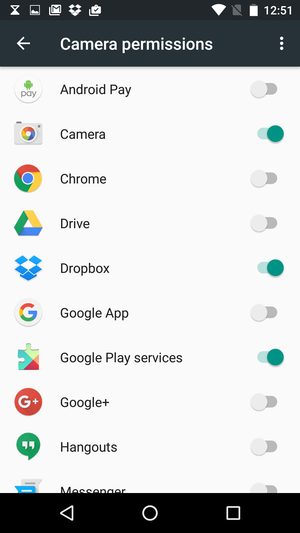
\includegraphics[width=3.5cm]{img/permissions-android.png}
    \par\end{center}
  \end{columns}
\end{frame}

\begin{frame}
    \frametitle{Vertrauenswürdige Software?}
    \begin{center}\Large
        Einer Software, die nicht quelloffen ist, kann man nicht vertrauen
    \end{center}
\end{frame}

\begin{frame}{Freie Software auf dem Smartphone}
  \begin{columns}
    \column{6.5cm}

    \textbf{F-Droid}\\
    Android-Appstore für freie Software

    \vspace{0.5cm}

    \textbf{iOS Open Source Apps}\\
    \url{https://github.com/dkhamsing/open-source-ios-apps}

    \column{5cm}

    \begin{center}
      
\includegraphics[width=2cm]{img/F-Droid_Logo_2}
    \par\end{center}
    \begin{center}
    \par\end{center}
  \end{columns}
\end{frame}

\begin{frame}{Replicant (Alternativ: Cyanogenmod)}
  \begin{columns}
    \column{6cm}
    \begin{itemize}
      \item basiert auf Android
      \item Ziel, alle proprietären Komponenten durch freie zu ersetzen
      \item Einbindung von F-Droid
      \item \textbf{Problem:} Verlust der Garantie bei Installation
    \end{itemize}
    \column{5cm}
    \begin{center}
      
\includegraphics[width=2cm]{img/Replicant_logo_alpha}
    \par\end{center}
  \end{columns}
\end{frame}

\begin{frame}
  \frametitle{Ubuntu Phone, Sailfish OS}
    \begin{center}
      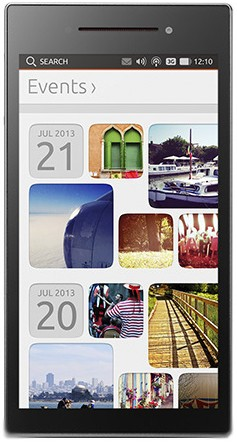
\includegraphics[height=6cm]{img/ubuntuphone.jpg}
      \hspace{0.5cm}
      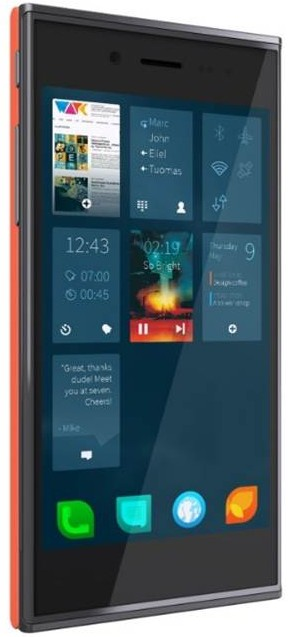
\includegraphics[height=6cm]{img/sailfishos.jpg}
    \end{center}
\end{frame}

\begin{frame}{Geräteverschlüsselung}
  \begin{columns}
    \column{5.5cm}
    \footnotesize

    \textbf{Android}\\
    Standard ab 6.0
    Einstellungen -> Sicherheit -> Telefon verschlüsseln\\
    \vspace{0.5cm}

    \textbf{iOS}\\
    Standard\\
    \vspace{0.5cm}
    \textbf{wichtig:} gute PIN/Muster

    \column{5cm}

    \begin{center}
      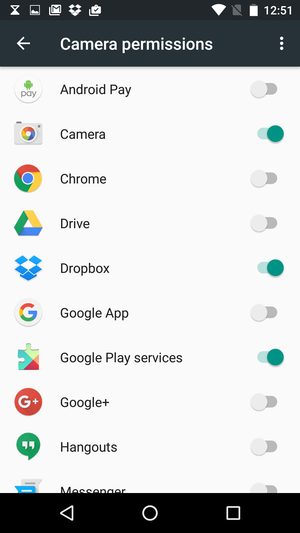
\includegraphics[width=3.5cm]{img/permissions-android.png}
    \par\end{center}
  \end{columns}
\end{frame}

\begin{frame}
    \frametitle{Was ist zu schützen?}
    \begin{center}
      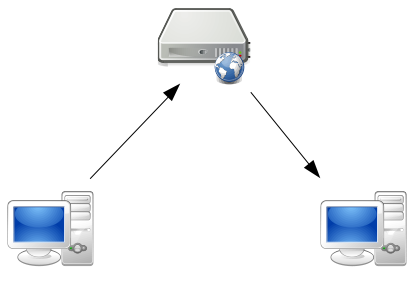
\includegraphics[height=5cm]{img/c-s.png}
    \end{center}
\end{frame}

\section{Inhalte}
\subsection{}

\begin{frame}
    \frametitle{Tempora}
    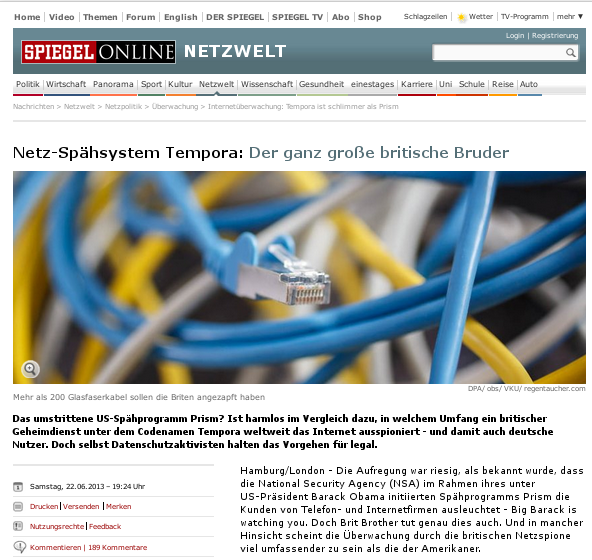
\includegraphics[height=0.7\textheight]{img/spiegel-tempora.png}
\end{frame}

\begin{frame}
    \frametitle{Transportwegverschlüsselung}
      SSL = Secure Socket Layer / TLS = Transport Layer Security
    \vfill
    \begin{center}
      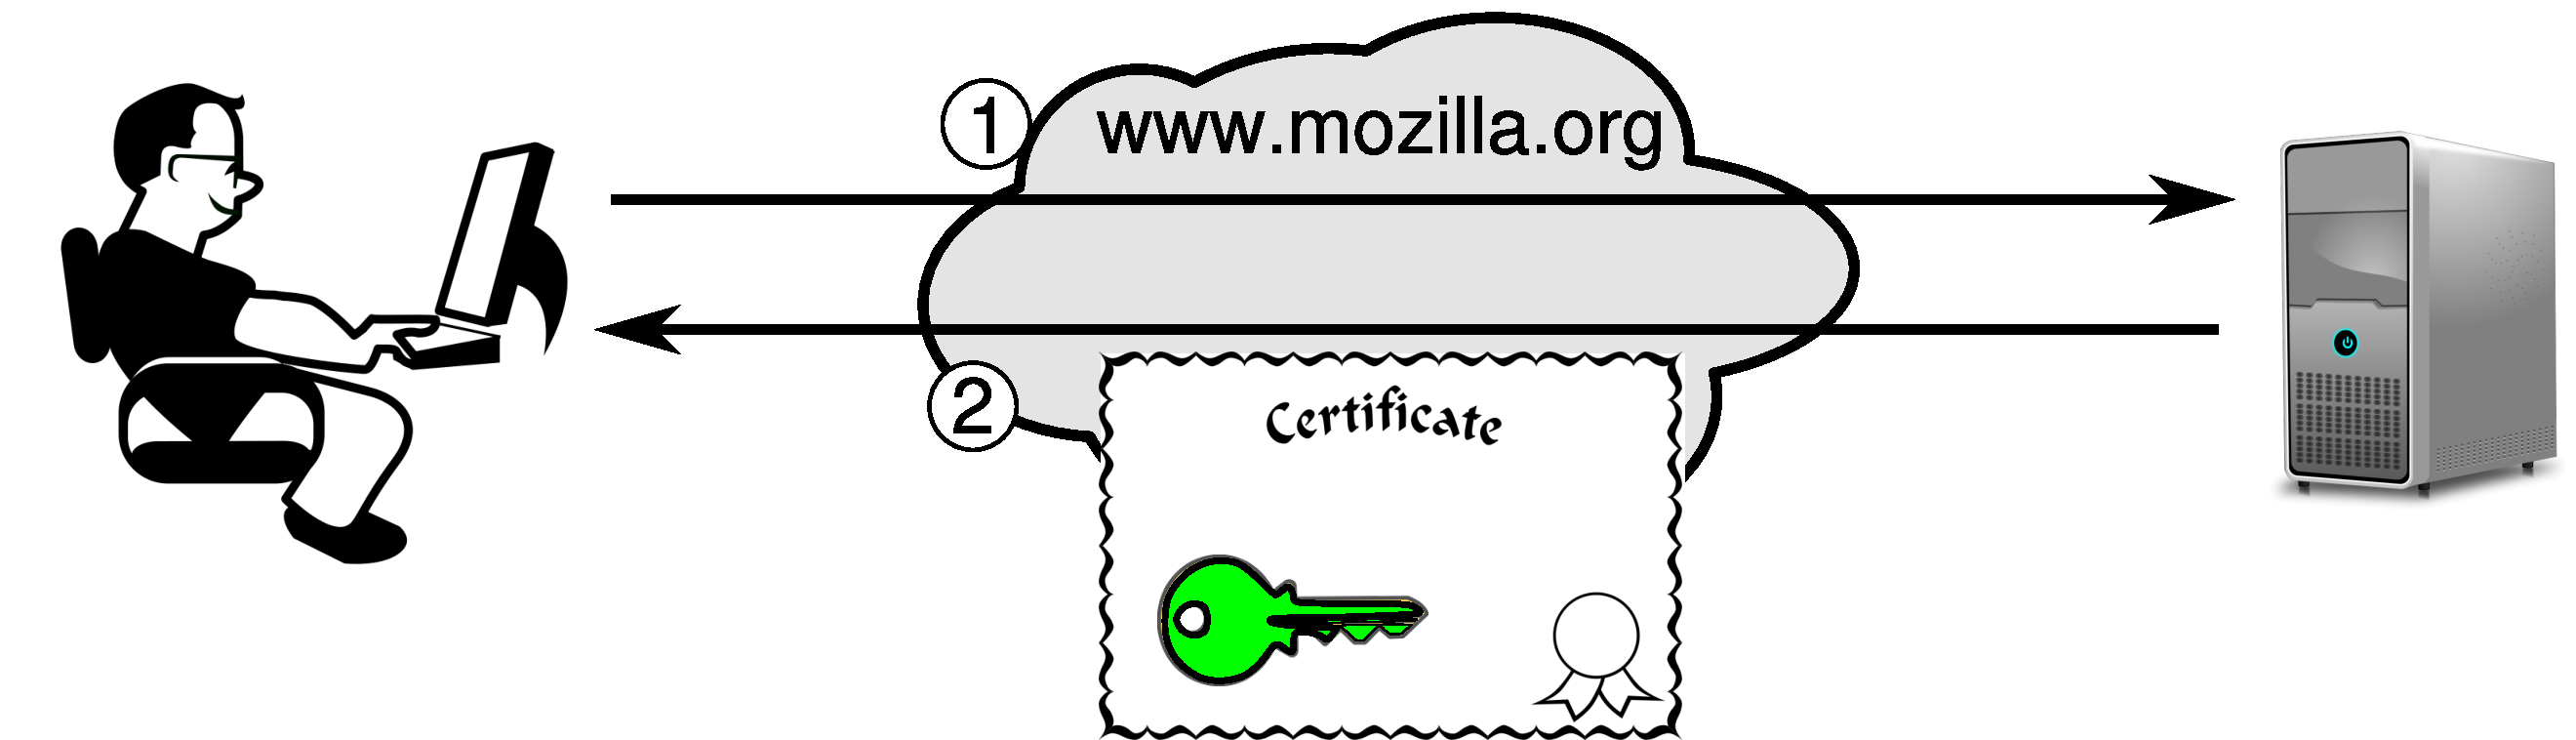
\includegraphics[width=0.8\textwidth]{img/tls.pdf}
    \end{center}
\end{frame}

\begin{frame}
    \frametitle{SSL im Browser}
    \begin{center}
	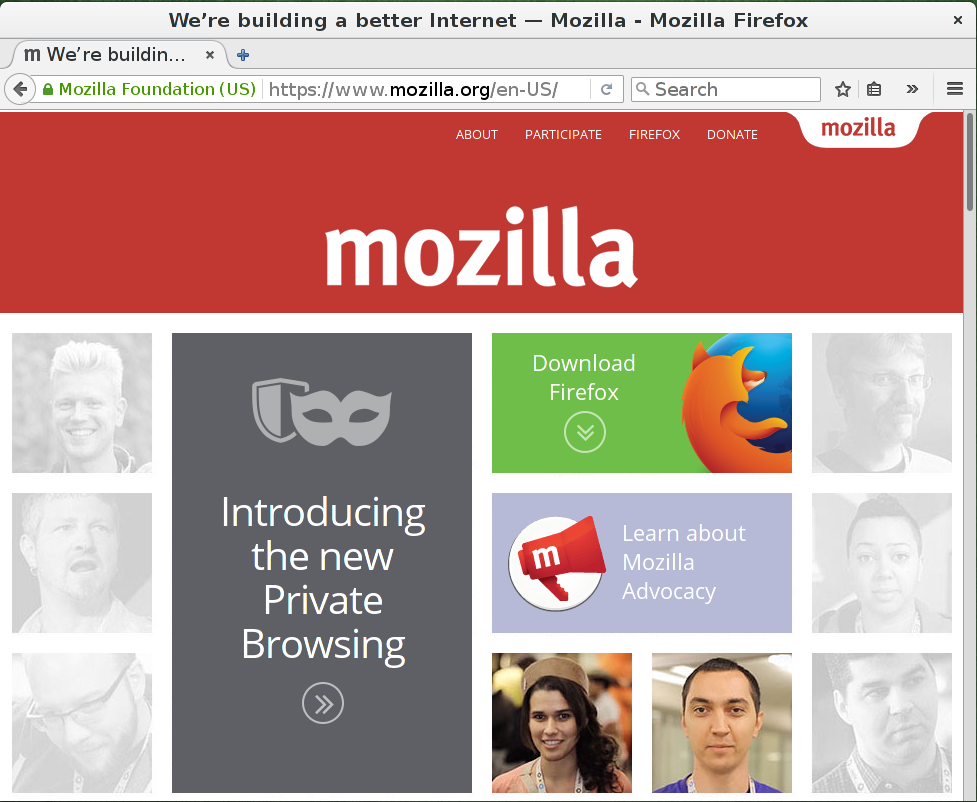
\includegraphics[height=0.7\textheight]{img/ssl_special.png}
    \end{center}
\end{frame}

\begin{frame}
    \frametitle{Ungültiges Zertifikat}
    \begin{center}
	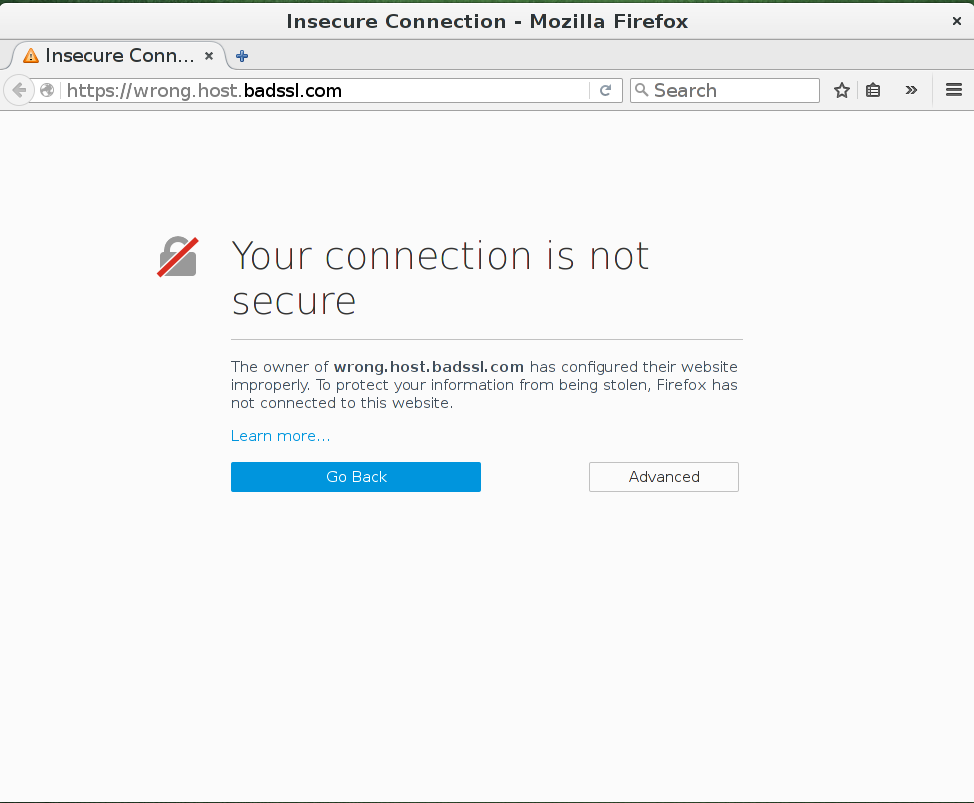
\includegraphics[height=0.7\textheight]{img/ssl_badcert.png}
    \end{center}
\end{frame}

\begin{frame}
    \frametitle{Was ist zu schützen?}
    \begin{center}
      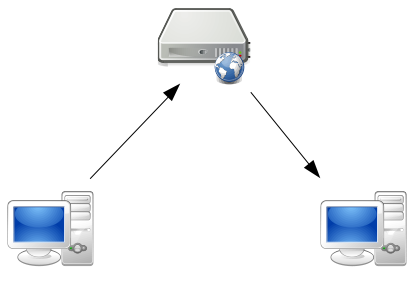
\includegraphics[height=5cm]{img/c-s.png}
    \end{center}
\end{frame}

\begin{frame}
    \frametitle{Prism}
    \begin{center}
      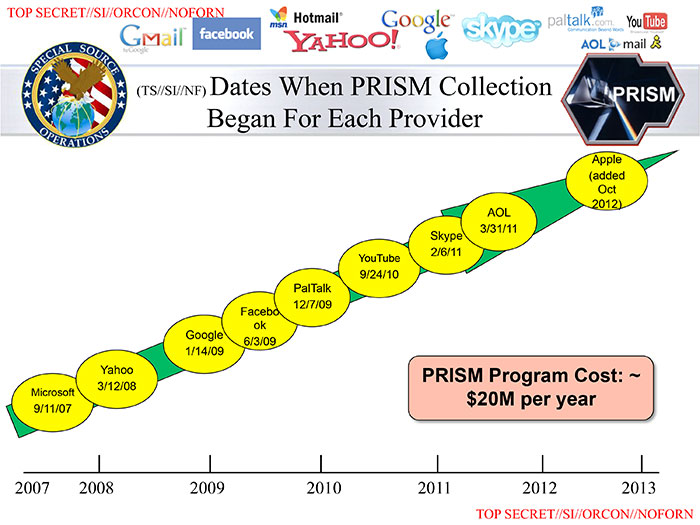
\includegraphics[height=0.7\textheight]{img/prism.jpg}
    \end{center}
\end{frame}

\begin{frame}
  \frametitle{Dezentrale Dienste}
    \begin{columns}
        \begin{column}{5cm}
            \begin{center}
                
\includegraphics[height=0.2\textheight]{img/mail.pdf} \\
                E-Mail \\
                \vspace{1cm}
                
\includegraphics[height=0.2\textheight]{img/jabber.png}
            \end{center}
        \end{column}
        \begin{column}{5cm}
            \begin{center}
                
\includegraphics[height=0.2\textheight]{img/owncloud.png} \\
                \vspace{1cm}
                
\includegraphics[width=0.8\textwidth]{img/sandstorm.png}
            \end{center}
        \end{column}
    \end{columns}
\end{frame}

\begin{frame}{Owncloud}
  \begin{columns}
    \column{4cm}
    \footnotesize

    Plattformübergreifende Synchronisierung von Dateien, Dokumenten, Kalendern, Kontakten, Notizen und News.

    \column{6cm}

    \begin{center}
      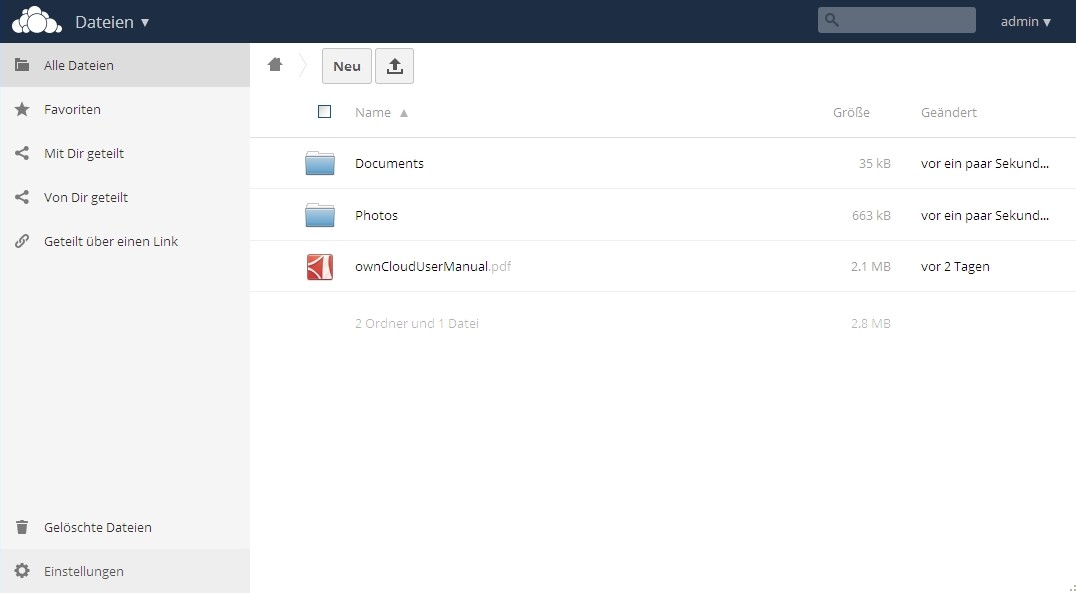
\includegraphics[width=6cm]{img/owncloud-screenshot.jpg}
    \par\end{center}
  \end{columns}
\end{frame}

\begin{frame}
  \frametitle{Ende-zu-Ende-Verschlüsselung}
  \begin{itemize}
    \item<1-> GPG für E-Mails
    \item<2-> OTR/OMEMO für Jabber:
      \begin{itemize}
        \item Pidgin mit OTR-Plugin für Linux und Windows
        \item ChatSecure oder Xabber für Android
        \item Adium für Mac, ChatSecure für iOS
      \end{itemize}
    \item<3-> palava.tv, talky.io, Tox, Linphone für Videotelefonie
    \item<4-> Signal
  \end{itemize}
\end{frame}

\begin{frame}
  \frametitle{Jabber: Conversations, ChatSecure}
    \begin{center}
      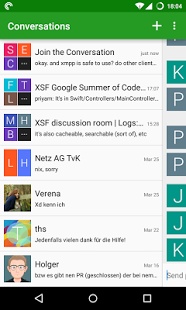
\includegraphics[height=6cm]{img/conversations.png}
      \hspace{0.5cm}
      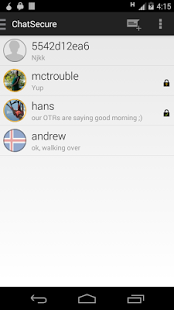
\includegraphics[height=6cm]{img/chatsecure.png}
    \end{center}
    \url{https://xmpp.net/directory.php}
\end{frame}

\begin{frame}
  \frametitle{Signal}
    \begin{center}
      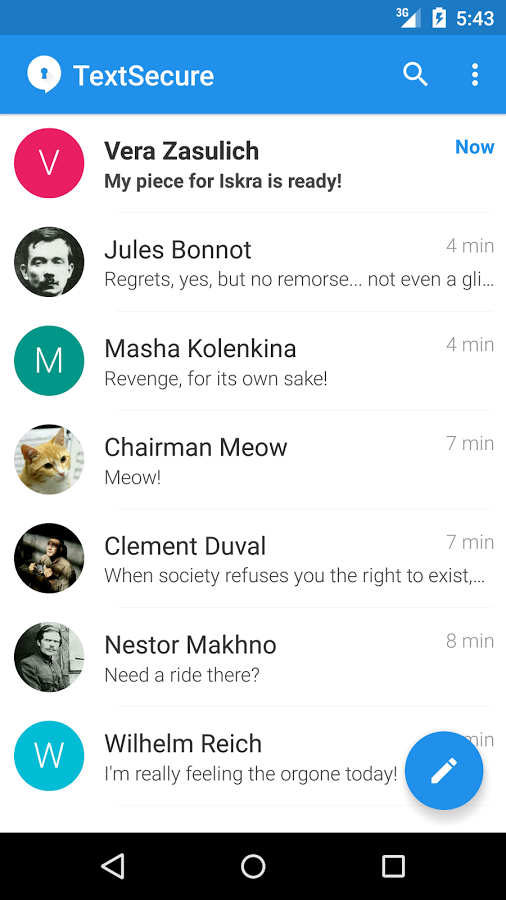
\includegraphics[height=6cm]{img/signal1.png}
      \hspace{0.5cm}
      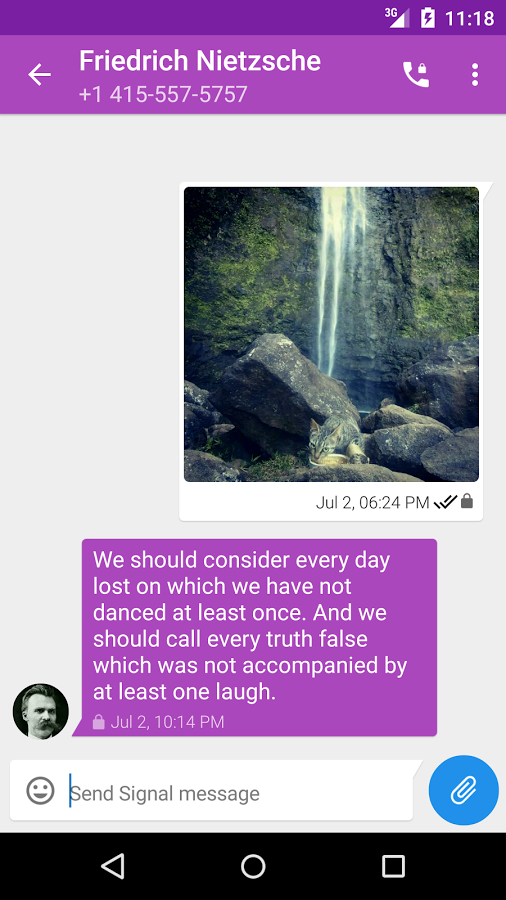
\includegraphics[height=6cm]{img/signal2.png}
    \end{center}
\end{frame}

% TODO Vergleichstabelle Messenger

\begin{frame}
  \frametitle{Vergleich Messenger}
  \small
  \begin{tabular}{|c|c|c|c|c|c|}
    \hline
                      & Whatsapp            & Threema             & Telegram              & Signal                & Jabber              \\
    \hline
    Verschlüsselung   & \cellcolor{orange}  & \cellcolor{yellow}  & \cellcolor{orange}    & \cellcolor{green}     & \cellcolor{green}   \\
    \hline
    Vertrauensw.      & \cellcolor{red}     & \cellcolor{yellow}  & \cellcolor{orange}    & \cellcolor{green}     & \cellcolor{green}   \\
    \hline
    Dezentr.          & \cellcolor{red}     & \cellcolor{red}     & \cellcolor{red}       & \cellcolor{orange}    & \cellcolor{green}   \\
    \hline
    Open Source       & \cellcolor{red}     & \cellcolor{red}     & \cellcolor{yellow}    & \cellcolor{green}     & \cellcolor{green}   \\
    \hline
    Mobileignung      & \cellcolor{green}   & \cellcolor{green}   & \cellcolor{green}     & \cellcolor{green}     & \cellcolor{yellow}  \\
    \hline
  \end{tabular}
\end{frame}

\begin{frame}
  \frametitle{Was kümmert es Facebook, Google und co?}
    \begin{center} 
      \includegraphics<1>[width=0.7\textwidth]{img/facebookgoogleencryption.png}
    \end{center}
\end{frame}

\section{Metadaten}
\subsection{}

\begin{frame}
    \frametitle{Tracking}
    \begin{center} 
        \includegraphics<1>[width=0.7\textwidth]{img/lightbeam_1.png}
        \includegraphics<2>[width=0.7\textwidth]{img/lightbeam_2.png}
    \end{center}
\end{frame}

\begin{frame}
  \frametitle{Metadaten - Vorratsdatenspeicherung}
  \begin{itemize}
    \item Handynetz
      \begin{itemize}
        \item Telefonnummern
        \item Zeitpunkt und Dauer (Telefonate, SMS)
        \item Funkzelle (Ort)
      \end{itemize}
    \item Internet
      \begin{itemize}
        \item IP-Adresse (= ungefährer Ort)
        \item Alle Verbindungen
        \item Email: Adressen von Sender und Empfänger, Zugriff
      \end{itemize}
  \end{itemize}
\end{frame}

\begin{frame}
    \frametitle{Metadaten}
    \begin{center}
      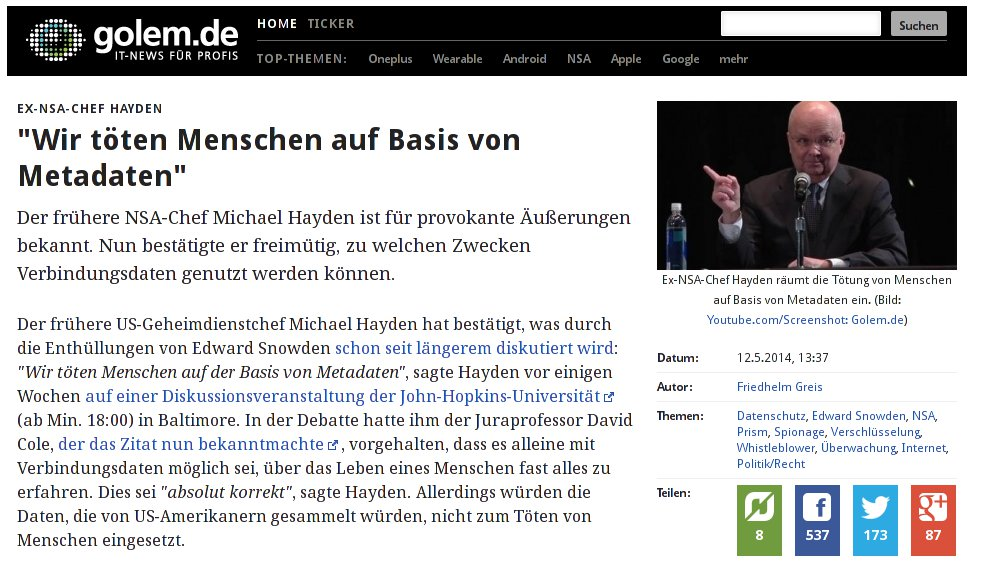
\includegraphics[height=0.7\textheight]{img/wekillpeople.jpg}
    \end{center}
\end{frame}

\begin{frame}
    \frametitle{Metadaten - VDS}
    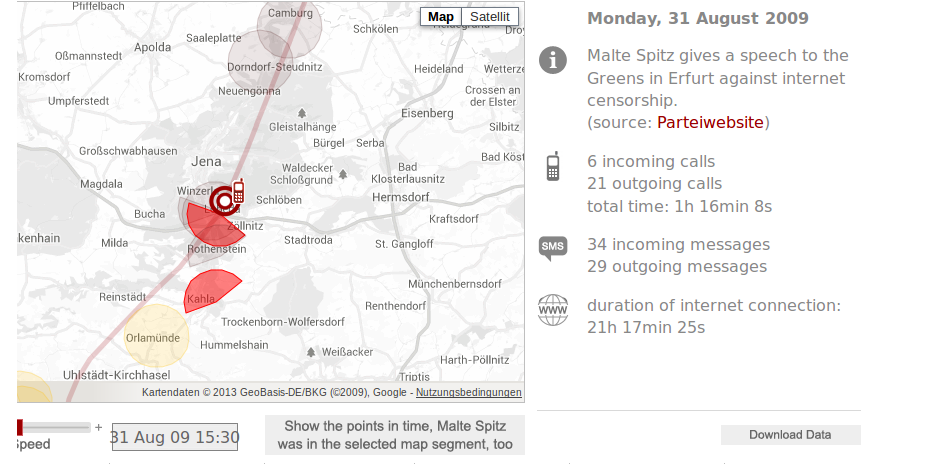
\includegraphics[height=0.7\textheight]{img/maltespitz.png}
\end{frame}

\begin{frame}
    \frametitle{Google Takeout}
    \begin{center}
      \includegraphics[width=0.8\textwidth]<1>{img/google_heat_1.png}
      \includegraphics[width=0.8\textwidth]<2>{img/google_heat_2.png}
    \end{center}
\end{frame}

\begin{frame}
    \frametitle{Zeitstempel}
    \begin{center}
      \only<1>{
        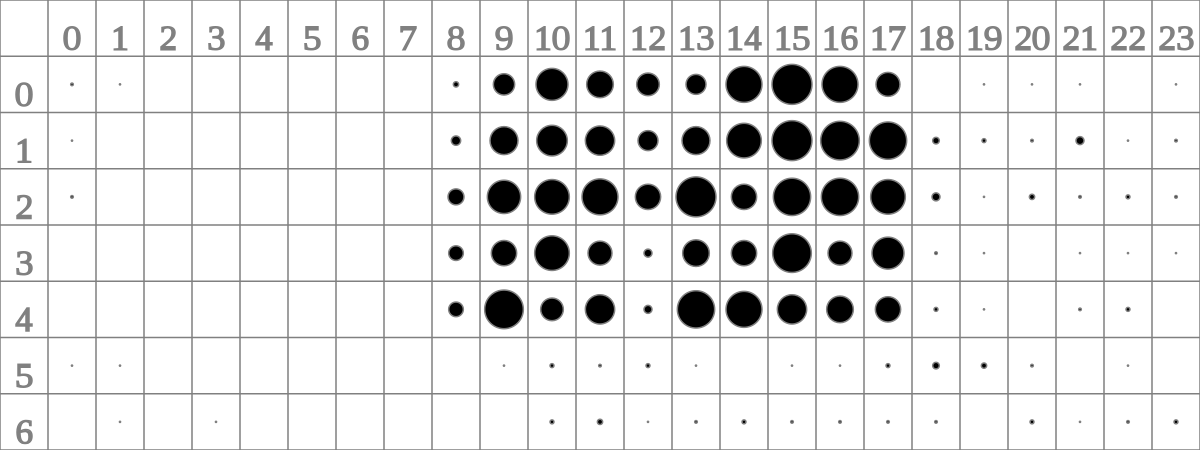
\includegraphics[width=0.9\textwidth]{img/punch_1.png}
        \\ \hfill \small Alan, Microblogging
      }

      \only<2>{
        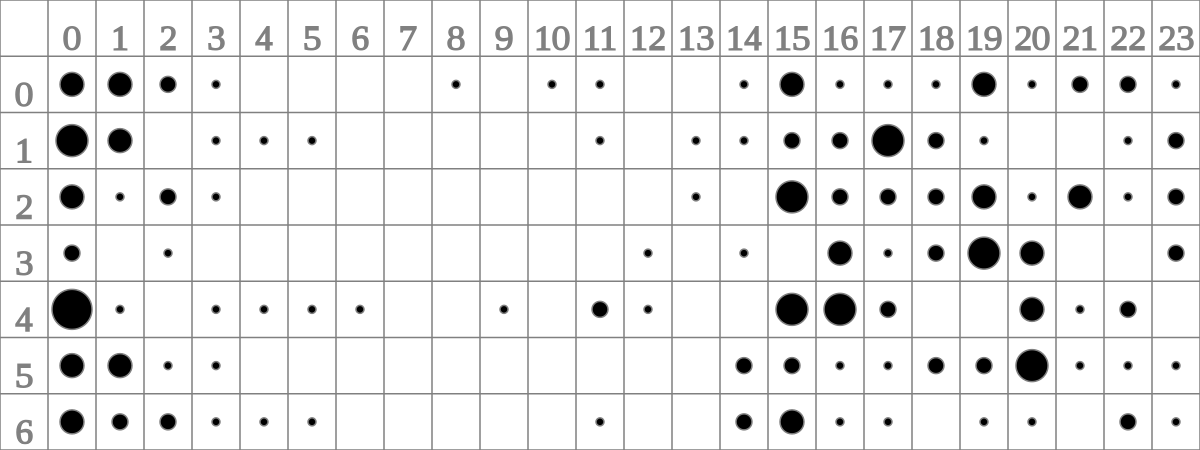
\includegraphics[width=0.9\textwidth]{img/punch_2.png}
        \\ \hfill \small Bob, Microblogging
      }

      \only<3>{
        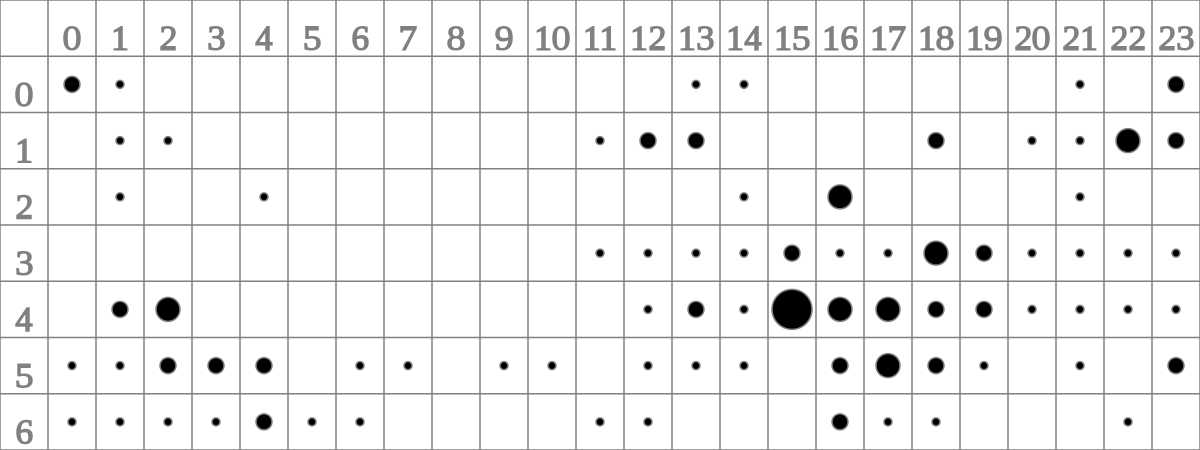
\includegraphics[width=0.9\textwidth]{img/punch_3.png}
        \\ \hfill \small Charlie, Github
      }
    \end{center}
\end{frame}

\begin{frame}{Antitracking für den Browser}
  \textbf{Computer}\\
  Browser-Plugins: Disconnect, Privacy Badger\\
  \vspace{0.5cm}

  \textbf{Smartphone}\\
  Bislang keine Open Source Apps, Privacy Badger in Arbeit
\end{frame}

\begin{frame}{Antitracking für Apps}
  \begin{columns}
    \column{5.5cm}
    \footnotesize

    \textbf{Android: Google AdID}\\
    Google-Einstellungen -> Anzeigen -> Anzeigen\\
    \vspace{0.5cm}

    \textbf{iOS: Apple IDFA}\\
    Settings -> General -> About -> Advertising\\
    \vspace{0.5cm}

    \column{5cm}

    \begin{center}
      \includegraphics[width=3.5cm]{img/google-adid.png}
    \par\end{center}
  \end{columns}
\end{frame}

\begin{frame}
  \frametitle{Tor (Orbot/Orweb, OnionBrowser)}
    \begin{center}
      \includegraphics[height=6cm]{img/orbot.png}
      \hspace{0.5cm}
      \includegraphics[height=6cm]{img/onionbrowser.png}
    \end{center}
\end{frame}

\begin{frame}
    \frametitle{Tor}
    \includegraphics[height=0.7\textheight]{img/tor1.png}
    \\{\small \href{https://www.torproject.org/images/htw1.png}{Grafik}: \href{https://creativecommons.org/licenses/by/3.0/us/}{\cc{by}} The Tor Project}
\end{frame}

\begin{frame}
    \frametitle{Tor}
    \includegraphics[height=0.7\textheight]{img/tor2.png}
    \\{\small \href{https://www.torproject.org/images/htw2.png}{Grafik}: \href{https://creativecommons.org/licenses/by/3.0/us/}{\cc{by}} The Tor Project}
\end{frame}

\begin{frame}
    \frametitle{Tor}
    \includegraphics[height=0.7\textheight]{img/tor3.png}
    \\{\small \href{https://www.torproject.org/images/htw3.png}{Grafik}: \href{https://creativecommons.org/licenses/by/3.0/us/}{\cc{by}} The Tor Project}
\end{frame}

\section{Verhalten}
\subsection{}

\begin{frame}
    \frametitle{Passwörter}
    \begin{itemize}
        \item<2-> Keine einfachen Wörter
        \item<3-> Groß-, Kleinbuchstaben, Ziffern, Sonderzeichen
        \item<4-> Beispiele:
            \begin{itemize}
                \item<5-> dragon
                \item<6-> (nCuAj.§Tsm!f
                \item<7-> IchLiebeDich
                \item<8-> .§)=/)=`
                \item<9-> qwerty
                \item<10-> Mks?o/.u,1Psw!
            \end{itemize}
        \item<12-> Verschiedene Passwörter nutzen!
        \item<13-> Passwort-Manager verwenden \\ (z.B. Keepass, Password Safe)
    \end{itemize}
\end{frame}

\section{Fazit}
\subsection{}

\begin{frame}
  \frametitle{Fazit}
  \begin{center}
    \begin{itemize}
      \item Verschlüsselung nutzen (Signal, Conversations, ChatSecure)
      \item Anonymisieren (Antitracking-Einstellungen, Tor)
      \item Dezentrale Dienste nutzen (Email, Jabber, Owncloud)
      \item Endgeräte schützen (Permissions, Freie Software, Geräteverschlüsselung)
    \end{itemize}

    \vspace{5mm}
    \href{https://github.com/c3d2/cms}{Folien}: \href{https://creativecommons.org/licenses/by-sa/4.0/}{\cc{by-sa}} Chaos Computer Club Dresden \\
    \vspace{3mm}
    CMS Dresden: schule@c3d2.de\\
    Vortragender: Marius Melzer (marius@rasumi.net, PGP-Fingerprint: 6730 E691 36B9 9BB8 FFB1 2662 A97B F176 52DE FC3E)
  \end{center}
\end{frame}

\end{document}
